% 英文で執筆する場合はクラスファイルへのオプションを[T,E]としてください.
% If you want to write your paper in English, pass to [T,E] options to document class.
\documentclass[T,J]{fose} % 「コンピュータソフトウェア」用のクラスファイルは compsoft です.
\taikai{2024} % 固定です.出版委員長が毎年変更してAuthor Kitを配布してください.

\usepackage [dvipdfmx] {graphicx}
\usepackage{xcolor} % 色を扱うためのパッケージ
% ユーザが定義したマクロなどはここに置く.ただし学会誌のスタイルの
% 再定義は原則として避けること.

% 以下は説明のために使用したパッケージであるため,削除可能.
\usepackage{listings}
\usepackage{tabularx}
\usepackage{fancyvrb}
\usepackage{xurl}
\usepackage{cite}
\usepackage[dvipdfmx]{graphicx}
\usepackage{latexsym}
\usepackage[T1]{fontenc}
\usepackage{lmodern}
\usepackage{textcomp}
\usepackage{latexsym}
\usepackage{url}
\usepackage{multirow}
% 以下のマクロはサンプルファイル作成用のマクロです.不要であれば削除してください.
\newcommand{\foseclassfile}{fose.cls}
\newcommand{\fosestylefile}{fose.sty}
\newcommand{\todo}[1]{\colorbox{yellow}{{\bf TODO}:}{\color{red} {\textbf{[#1]}}}}
\newcommand{\change}[1]{\colorbox{green}{{\bf CHANGE}:}{\color{red} {\textbf{[#1]}}}}

\begin{document}

% 論文のタイトル クライアントのソフトウェア(コード),パターン特定手法,影響範囲特定,
%後方互換性の損失に関係する使用パターンをもとにしたライブラリクライアントへの影響範囲の特定    
%後方互換性の損失におけるライブラリクライアントへの影響範囲の特定
%クライアントコードに基づく後方互換性の損失の影響範囲の特定
\title{JavaScriptライブラリの後方互換性の損失によるクライアントへの影響範囲の特定}
% 以下の \etitle(と\@etitle)はFOSE論文フォーマット独自のマクロです.
% FOSEに投稿した論文を発展させてコンピュータソフトウェアに投稿される場合はコメントアウトしてください.
% \setetitleは奇数ページのヘッダに表示する文字列(\etitle)を設定するためのマクロです.
% タイトルが2行に渡る場合は "\\" を 使用することで任意の位置で改行をすることができます.
\setetitle{Identification of Clients due to Loss of JavaScript Library Backward Compatibility}
%\setetitle{Long Long Long Long Long Long \\ Long Long Long Long Long \\ Long Long Long Long Long Long Long Long Long Long Long Long Paper Title}

% タイトル,著者などが複数行にわたり,論文冒頭の著者名が日本語アブストと重複して描画された場合に以下のコメントアウトを外してください.
%\longtitle

% 著者
% 和文論文の場合,姓と名の間には半角スペースを入れ,
% 複数の著者の間は全角スペースで区切る
%
\author{飯田 智輝 伊原 彰紀
%
% ここにタイトル英訳 (英文の場合は和訳) を書く.
% 英語タイトルは論文1ページ目左下,著者らの名前・所属一覧の一番上に表示される
%
% 上記\setetitle中で改行した場合は "\etitle" を削除し,改行(\\)を入れていないタイトルを記載してください.
% \ejtitleは1ページ目左下に挿入されるタイトルとして使用されます.
% また,"\etitle"はFOSE論文フォーマット独自のマクロです.
\ejtitle{\etitle}
%
% ここに著者英文表記 および
% 所属 (和文および英文) を書く.
% 複数著者の所属はまとめてよい
% 複数著者の所属は以下のようにまとめてよい.
\shozoku{Tomoki Iida, Akinori Ihara}{和歌山大学}
{Wakayama University}
}
%
% 和文アブストラクト

% In English paper, content of Jabstract will be ignored. 
\Jabstract{%
ソフトウェア開発では,開発効率を上げるために特定の機能がまとめられたライブラリを利用する.ライブラリ開発者がライブラリの品質を維持するために機能追加や修正などを行いバージョン更新する中で,既存機能の変更や削除によって後方互換性を損失することがある.後方互換性の損失はライブラリを利用するクライアントソフトウェアの振る舞いの阻害につながるが,ライブラリ開発者がクライアントソフトウェアを実行することなく影響範囲を特定することは容易ではない.本研究では,ライブラリ更新後にクライアントテストが失敗となったクライアントから依存ライブラリに関わるソースコード断片を抽出し,後方互換性の損失の原因となるソースコード断片からライブラリと関数の呼び出し分の記述パターンを作成する.作成した記述パターンをもとにテストが成功しているクライアントを分析することで,実際には影響を受けているクライアントを特定する.
}
%
% 英文アブストラクト(本サンプルの原論文にはなし)
% \Eabstract{
% This document has been prepared as a sample for FOSE(Foundation of Software Engineering) based on the Author Kit for rePiT and FOSE2022.
% The author kit for rePiT was originally based on author kit of JSSST Computer Software.
% The detail changes are written in Sec.\ref{sec:PaperStyle}
% }
%
\maketitle \thispagestyle {empty}

%%%%%%%%%%%%%%%%%%%%%%%%%%%%%
\section{はじめに}
%%%%%%%%%%%%%%%%%%%%%%%%%%%%%

ソフトウェア開発を効率的に進めるために機能が使いやすい形にまとめられたライブラリが広く公開されている.開発者はライブラリの利用により,開発者自身が同じ機能を再実装する必要がなくなるため開発効率が向上する.\cite{konstantopoulos2009best}\cite{Moser1996effect}.ソフトウェアが新機能追加,バグ修正によって頻繁にソースコードを更新されるように,ライブラリも例外ではない.\cite{raemaekers2012measuring}.ライブラリの更新には,脆弱性の修正などライブラリを利用するクライアントソフトウェア(以降,クライア
ント)にとって重要な変更が含まれることがあり,ライブラリのバージョン更新は,ライブラリを再利用するクライアントが依存ライブラリの更新を余儀なくされることも多い.

ライブラリのバージョン更新はソフトウェアの品質維持のために重要であるが,ライブラリ更新に機能削除や仕様変更といったクライアントに影響を与える変更が含まれる場合,更新前後でライブラリのソースコードに不整合が生じ,クライアントが実行時エラーになることがある.このように,更新後の依存ライブラリがクライアントに影響を与えることを後方互換性を損失するという.通常は,後方互換性を損失するバージョンをリリースする場合,バージョン名で後方互換性を損失する変更を含むことが周知できるようメジャーバージョンとしてリリースする.しかし,バージョン名の付与はライブラリ開発者が手動で行うため,後方互換性を損失しているにもかかわらず誤ってマイナーバージョンとしてリリースすることもあり,当該変更に関して機能の動作変更内容が文書化されていないことがある\cite{mostafa2017experience}.

Mujahidらは,後方互換性を損失するJavaScriptライブラリバージョンを特定するために,ライブラリ適用前後のクライアントテストを確認する実験を行っている\cite{mujahid}.当該研究は,クライアントテストの成否をもとに影響を受けたクライアントを把握しているが,クライアントテストが不十分な場合に後方互換性の損失の影響を受けていることを検出できない.事前分析としてuuidの2つのバージョンを調査した結果,後方互換性を損失する多くのライブラリは,ライブラリの呼び出し文と関数の呼び出し文を変更しており,本研究ではライブラリと関数の呼び出し文と関数の呼び出し文の記法に着目する.ただし,本研究の事前分析において,後方互換性を損失する場合ライブラリの呼び出し文と対応する関数の呼び出し文が多様であることを明らかにした.本研究では,多様なライブラリの呼び出し文を正規表現を用いて記述パターンを生成し,テストに成功したクライアントの中でライブラリの後方互換性の損失の影響を受けるクライアントを特定する.

% \color{red}
% 以降,本論文では,\ref{chap:intro}章でと従来研究について述べる.その後,\ref{chap:case_study}章でケーススタディのためのデータセットおよび分析方法を述べ,\ref{chap:result}章でRQ1,RQ2,RQ3の結果を述べる.そして,\ref{chap:disc}章で結果の考察および妥当性について述べ,\ref{chap:fig-tab-exp}章でまとめる.
% \color{black}

以降,本論文では,\ref{chap:intro}章で互換性の損失と従来研究について述べる.\ref{sec:method}章で後方互換性が損失するライブラリの呼び出し文,および関数呼び出し文の記述パターンの生成方法を述べる.\ref{chap:case_study}章でケーススタディのためのデータセットおよび分析結果を述べ,\ref{sec:conclusion}章でまとめる.




%開発を効率的に進めるために機能を使いやすい形にまとめられているライブラリが使用されている.ライブラリ開発者がライブラリの機能追加や機能のバグ修正による更新を通じてライブラリの品質を維持することによりライブラリのクライアントは,ライブラリ使用箇所にかけるコード記述や品質維持にかけるコストを減らすことができる.

% 一方で,ライブラリの更新に伴い後方互換性の損失が発生することがある.後方互換性の損失とは,ライブラリの更新において既存の機能が削除または変更されることによりバージョン更新前に使用できた機能がバージョン更新後に使用できなくなるというものである.

% クライアントは,後方互換性の損失により更新前とコードを変更していなくてもエラーになるというようにソフトウェアの振る舞いが阻害され,修正において原因の特定と修正を余儀なくされる.また,ライブラリ側の変更に関して機能の動作変更内容が文書化されていないことが多いという問題が明らかになっている\cite{mostafa2017experience}.これは,クライアントの後方互換性の損失の対応にかかるコストの増加につながる.

% 従来研究\cite{mujahid}では,javascriptのライブラリのクライアントテストをバージョン更新前後で実行して更新前にテスト成功し,更新後に失敗したクライアントがいた場合に後方互換性を損失したと判定する手法を提案している.従来研究のバージョン更新後にテストを失敗したクライアントには,後方互換性の損失に関係するライブラリの使用パターンが含まれている.また,テストの成否をもとに影響を受けたクライアントを把握することができるが,テスト成功に含まれている後方互換性の損失の影響を受けるコードを含んでいるが,テスト不十分によりテストが成功しているクライアントは,検出することができない.本研究では,使用パターンをテストを失敗したクライアントから抽出し,テストが成功したクライアントに当てることで,テスト不十分の影響を受けないライブラリの後方互換性の損失の影響を把握することを目指す.
%----------------------
\begin{figure*}[t]
\centerline{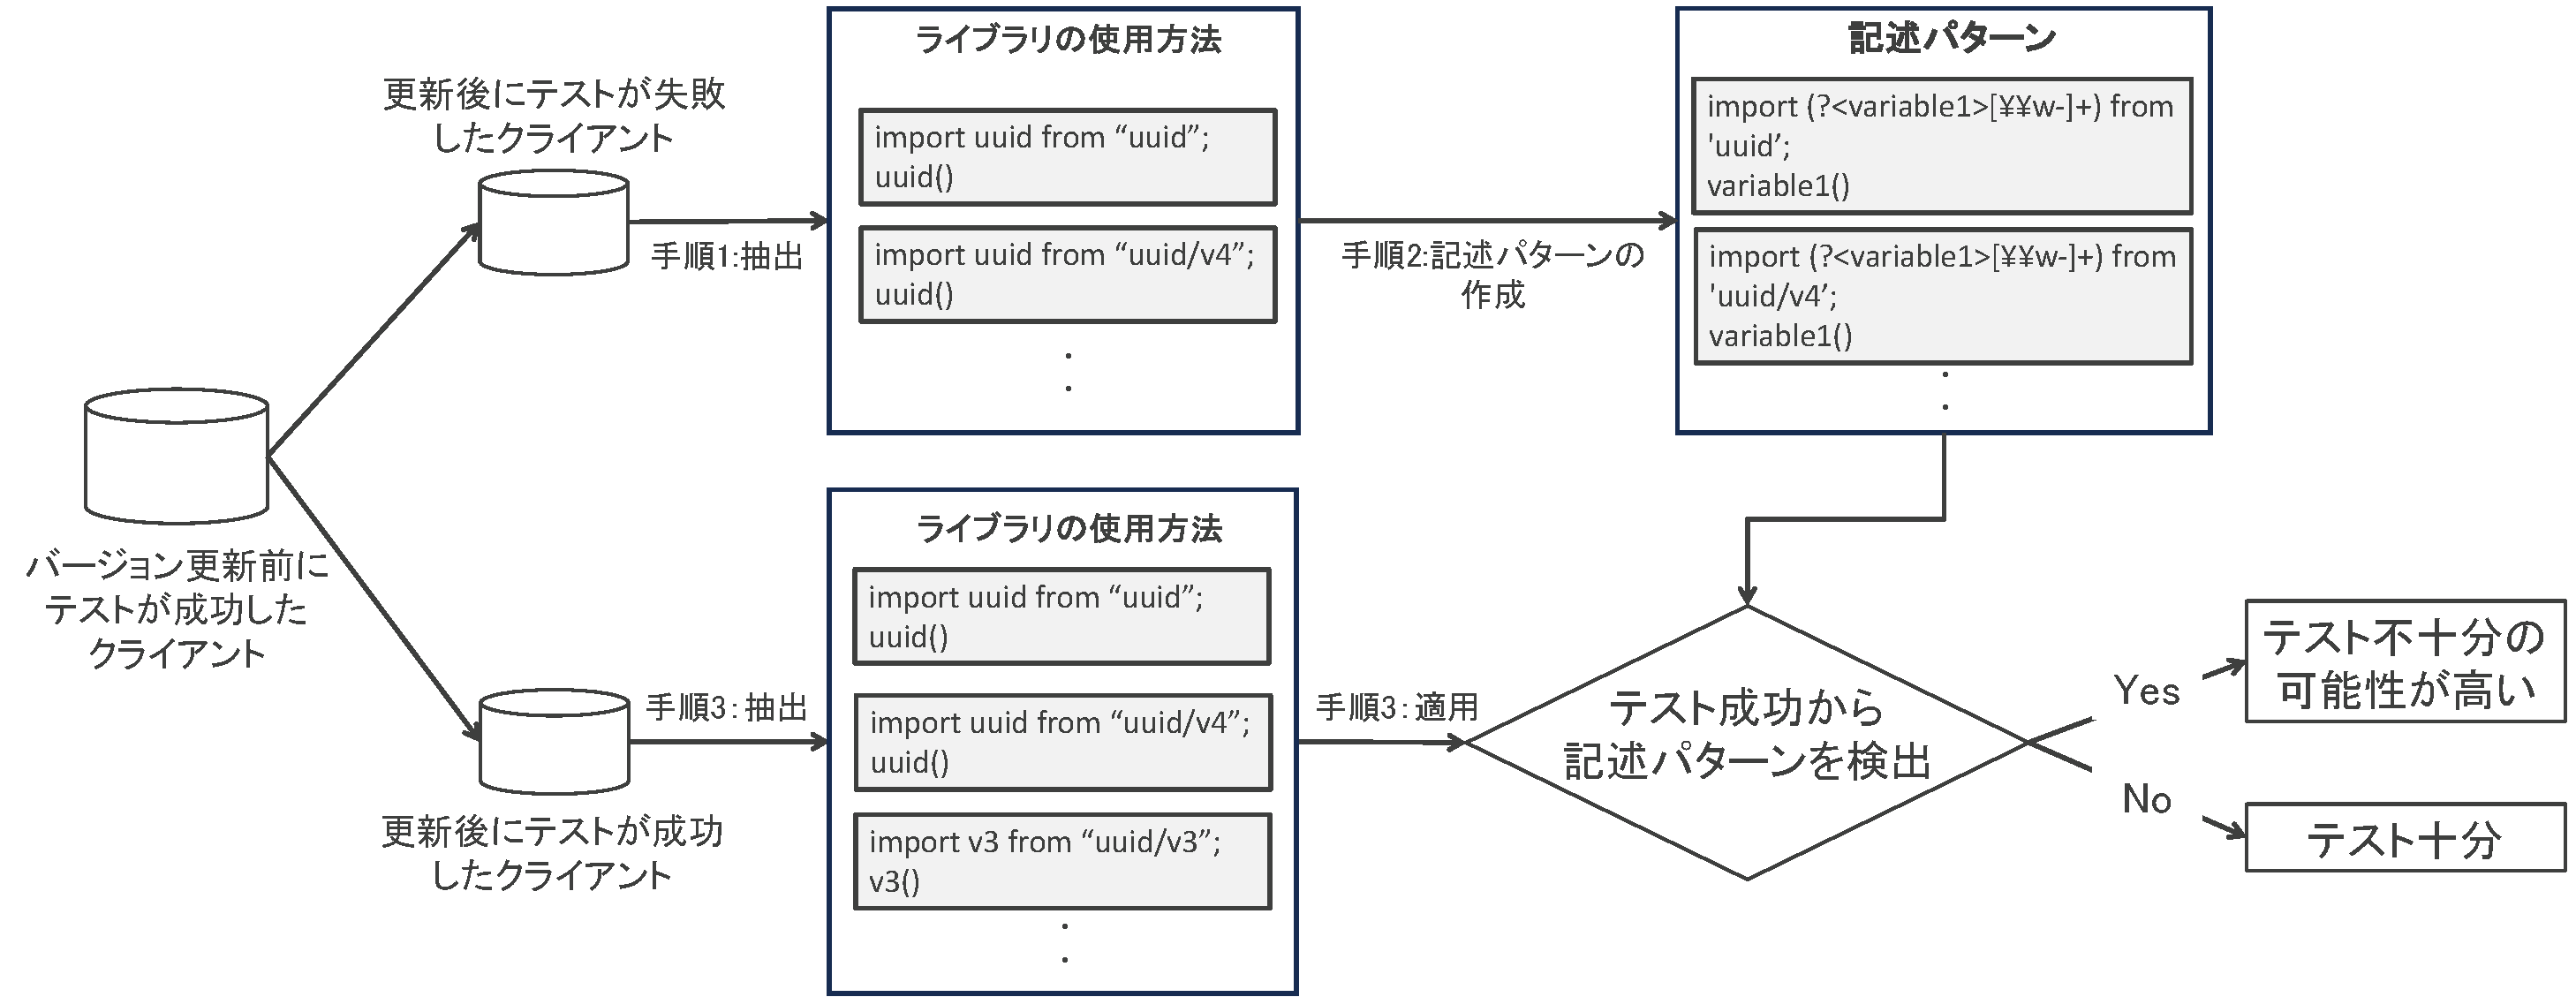
\includegraphics[width=1.0\linewidth]{Iida_fig/Fose_method.pdf}}
\caption{後方互換性の損失によるクライアントの特定手法の概略図}
\label{fig:method-overview}
\end{figure*}
%----------------------

%javascriptのライブラリバージョンのテスト変更の有無をもとに後方互換性の損失を判定し,mujahidらの\cite{mujahid}ライブラリバージョンにおけるクライアントテスト実行結果が更新後にテスト失敗になれば,後方互換性ありと判定する手法を同様のライブラリで行い検証に用いている手法がある.
%%%%%%%%%%%%%%%%%%%%%%%%%%%%%
\section{後方互換性の損失}\label{chap:intro}
%%%%%%%%%%%%%%%%%%%%%%%%%%%%%

\subsection{後方互換性の損失の課題}
ライブラリを利用することで効率的にソフトウェアを実装できるが,使用するライブラリバージョンの更新に後方互換性の損失が含まれるとクライアントが実行時エラーを引き起こすことがある.ライブラリバージョンに後方互換性の損失を含む場合,クライアントはライブラリのバージョンをダウングレードするか,後方互換性の損失の影響を受けない書き方に書き換えるか,または影響を受ける機能の使用を停止することになる.後方互換性の損失を含むライブラリをリリースする場合,ライブラリ開発者は影響を受けない書き方を公開することもあるが,既存機能の変更に関する文書化がされていないことが多く,開発者にとってライブラリの更新判断や修正にかけるコストが増加している\cite{mostafa2017experience}.

% ライブラリの更新に後方互換性の損失が含まれるとバージョンを更新したクライアントのソフトウェアがエラー等により実行できなくなるという問題を引き起こす.この時,クライアントは,ダウングレードまたは後方互換性の損失の原因をソースコードから特定し,新しい使い方への対応や削除を行う必要がある.ライブラリ開発者は,新しいバージョンリリースの際に情報を提供することはあるが後方互換性の損失の有無や変更内容の文書化が不足している.実際にjava言語のライブラリでは,既存機能の変更に関する文書化があまりされていないことが明らかになっている\cite{mosta}.これにより,ライブラリのクライアントがライブラリの更新判断や修正にかけるコストが増加している.

\subsection{従来研究}
ライブラリバージョンの更新における後方互換性の損失の有無を判定する手法としてテストを用いる手法が提案されている\cite{mujahid1}\cite{matsuda}.Mujahidらは,ライブラリの後方互換性の損失の有無を判定するために,該当ライブラリに依存するクライアントテストを用いた手法を提案している\cite{mujahid}.当該手法は,ライブラリバージョン更新前後でクライアントテストを実行し,成功していたテストが依存ライブラリの更新後に失敗すれば後方互換性の損失と判定する.また,松田らは,ライブラリの機能の変更に伴うライブラリのテスト変更の有無から後方互換性の損失の有無を判定する手法を提案しており,クライアントテストの実行結果をもとにした後方互換性の損失有無の判定を評価に利用している\cite{matsuda}.M{\o}llerらは,後方互換性の損失への対処を支援するために後方互換性の損失の影響を受けるクライアントのプログラムの場所を検出する手法を提案している\cite{10.1145/3428255}.この手法では,後方互換性の損失の影響を受ける記述パターン集を手作業で作成し,パターン集をもとにクライアントのソースコードを静的に解析することで影響を受ける場所を検出をしている.ただし,テストが成功しているクライアントの中で実際には後方互換性の損失の影響を受ける範囲は分析していない.
%\cite{10.1145/3428255:1}と自分の違いは,パターンを自動生成している点と正規表現を使う点

\subsection{動機}
ライブラリ開発者は,ライブラリの変更によってクライアントの振る舞いに影響を与えるライブラリの呼び出し方を確認することで,後方互換性の損失によるクライアントへの影響範囲を特定できる.しかし,ライブラリ更新のたびにクライアントのソースコードから使用方法を確認することはコストが膨大になるため現実的でない.
%さらに,ライブラリ開発者が後方互換性の損失を把握していない場合もある.更新前にクライアントへの影響を把握することも先ほどと同様の問題があるため現実的ではない.\todo{ここの書き方迷い中}

本研究では,依存ライブラリバージョンの更新に伴って後方互換性の損失の影響を受けたクライアントは,ライブラリが周知するライブラリの呼び出し方,関数の呼び出し方をしていたのか調査する.JavaScriptライブラリであるuuidで後方互換性の損失を含む2種類のバージョン更新(uuid@7.0.3...8.0.0-beta.0,uuid@3.4.0...7.0.0-beta.0\footnote{本論文ではバージョン更新前後のバージョン名を``更新前バージョン名...更新後バージョン名''と記す.})のいずれかを実施し,テストを失敗したクライアントにおけるライブラリの使用方法を目視調査した.バージョン8.0.0-beta.0および7.0.0-beta.0の後方互換性の損失に関係する呼び出し方はWebサイトに公開されている\footnote{https://github.com/uuidjs/uuid/blob/v7.0.0/\\CHANGELOG.md}\footnote{https://github.com/uuidjs/uuid/blob/v8.0.0/\\CHANGELOG.md}.ここで文書化されているのは,実際の失敗した原因の一部である.例えば,7.0.0-beta.0において「import * as uuid from ``uuid'', uuid();」の使い方は言及されていないがv8.0.0では使用できない呼び出し文である.本研究では,このようなライブラリ更新後にクライアントテストが失敗したクライアントから依存ライブラリに関わるソースコード断片を抽出し,後方互換性の損失の原因となるソースコード断片からライブラリと関数の呼び出し文の記述パターンを作成することで,後方互換性の損失の影響を受けるクライアントを特定する.

% uuid@7.0.3...8.0.0-beta.0のバージョン更新を実施したクライアント315件中47件で後方互換性を損失する呼び出し方法を使用していた.uuid@3.4.0...7.0.0-beta.0では436件中35件で後方互換性を損失する呼び出し方法を使用していた.テスト失敗した理由を調査した結果,テスト不十分が主な原因であり,その他はテスト実行不可,誤検出している事例を確認した.



% 確認作業のコストは大きいが,後方互換性の損失の影響を把握する方法として,クライアントテスト実行結果の成否から判断することができるが,テスト不十分なクライアントを影響を受けないと誤判定することもある.

% 本研究では,事前分析として後方互換性を損失するクライアントの

% プロジェクトが提供する後方互換性を損失するライブラリの呼び出し方法で実装するクライアントを目視調査した.

% JavaScriptライブラリであるuuidで後方互換性の損失を含む2種類のバージョン更新(uuid@7.0.3...8.0.0-beta.0,uuid@3.4.0...7.0.0-beta.0\footnote{本論文ではバージョン更新前後のバージョン名を``更新前バージョン名...更新後バージョン名''と記す.})のいずれかを実施し,テストを失敗したクライアントにおけるのライブラリの使用方法を目視調査した.uuidでは,後方互換性を損失する使用パターンを公開しており,それに従い

% uuid@7.0.3...8.0.0-beta.0のバージョン更新を実施したクライアント\todo{X件中}47件で後方互換性を損失する呼び出し方法を使用していた.uuid@3.4.0...7.0.0-beta.0では\todo{X件中}35件で後方互換性を損失する呼び出し方法を使用していた.テスト失敗した理由を調査した結果,テスト不十分が主な原因であり,その他はテスト実行不可,誤検出している事例を確認した.

% 使用パターンを作成のためにクライアントのソースコードを個別に確認することは

% ため作業があるため時間がかかり,,使用パターンをもとに検出する部分のコードを毎回変更する必要がある点も問題である.そこで,本研究では,更新後にテストを失敗したクライアントとテストが成功したクライアント,ライブラリ名を入力として使用パターンの作成から検出までを自動で行うことを目的とする.


%表\ref{table:dataset}のライブラリのuuid@7.0.3...8.0.0-beta.0,uuid@3.4.0...7.0.0-beta.0のテストを失敗したクライアントから目視で後方互換性の損失の影響を受ける使用パターンを特定し,テストが成功したクライアントに適用するということを行った.その結果,uuidの2例では,ライブラリ呼び出しと関数呼び出しの対応関係で使用パターンが定義できることがわかり,実際に使用パターンをもとに検出を行った結果uuid@3.4.0...7.0.0-beta.0で35件uuid@7.0.3...8.0.0-beta.0で47件が使用パターンを含むことがわかり,これらから10件ずつ検出したクライアントを確認したところ,uuid@3.4.0...7.0.0-beta.0では10件中テスト不十分が5件,テスト実行不可が2件,誤検出が2件,テストが失敗した1件であり,uuid@7.0.3...8.0.0-beta.0で10件ともテスト不十分であった.よって,誤検出のような考慮すべき点はあるが,テスト不十分やテストを実行できないクライアントを見つけることができると確認できた.しかし,目視で使用パターンを作成することコードを確認する作業があるため時間がかかり,,使用パターンをもとに検出する部分のコードを毎回変更する必要がある点も問題である.そこで,本研究では,更新後にテストを失敗したクライアントとテストが成功したクライアント,ライブラリ名を入力として使用パターンの作成から検出までを自動で行うことを目的とする.

%その結果,後方互換性を損失するソフトウェアでは,ライブラリの呼び出し文と引数を含む関数の呼び出し文に関係しており,本研究では2つの呼び出し文の書き方に着目する.また,ただし,本研究の\todo{事前分析?RQ1?}において,後方互換性の損失する場合ライブラリの呼び出し文が多様であることを明らかにした.本研究では,多様なライブラリの呼び出し文を正規表現を用いて命令パターンを生成し,テストに成功したクライアントの中でライブラリの後方互換性の損失の影響を受けるクライアントを特定する.


% バージョン更新に後方互換性の損失を伴う際に更新後に使用できなくなるライブラリの使用方法と影響を明らかにするためにバージョン更新前でクライアントテストが成功したクライアントをもとにバージョン更新後にテストが失敗したクライアントから更新後に使用できなくなる使用パターンの抽出と使用パターンをもとにテストを成功したクライアントへのパターンを含むか否かでの分類を行う.バージョン更新前にテストが成功していることから更新後テスト失敗したクライアントには,後方互換性の損失に関係するコードが含まれている.そのためテストを失敗したクライアントからは,使用パターンを抽出できる.そして,更新後にテストを成功していたクライアントがこの使用パターンを持っていれば,そのクライアントは実際は後方互換性の損失の影響を受けていると判断することができる.これにより,ライブラリ開発者がバージョン更新後の影響を考慮しながらのライブラリ開発を可能にするとともに使用パターンを更新後に使用できなくなる方法として文章化して情報を提供できるようになることを目指す.

%%%%%%%%%%%%%%%%%%%%%%%%%%%%%
\section{後方互換性の損失によるクライアントの特定手法}\label{sec:method}
%%%%%%%%%%%%%%%%%%%%%%%%%%%%%

本章では,依存ライブラリの更新に伴いテストが失敗したクライアントから後方互換性の損失の影響を受ける呼び出し文,および関数呼び出し文の記述パターンを生成する手法を述べる.図\ref{fig:method-overview}に後方互換性の損失によるクライアントの特定手法の概略図を示し,以降で各手順の説明を述べる.

%依存ライブラリに含まれる後方互換性の損失の影響を受ける呼び出し方であることが示唆される.本研究では,このような依存ライブラリの更新に伴いテストが失敗した多くのクライアントのソースコードから呼び出し文のパターンを生成\todo{作成?}する.

\noindent\textbf{手順1.テストが失敗したクライアントからライブラリの呼び出し文,関数呼び出し文を抽出}
クライアントのJavaScriptまたはTypeScriptで記述されたソースコードファイルを抽象構文木に変換し,ライブラリの呼び出し文(\texttt{import}文,\texttt{require}文),およびライブラリの関数呼び出し文を抽出する.

\noindent\textbf{手順2.ライブラリ呼び出し文,関数呼び出し文の記述パターンの生成}

ライブラリ呼び出し文,関数呼び出し文の変数名や関数名を抽象化したのち,正規表現として記述パターンを生成する.具体的には,図\ref{fig:method-overview}における変換は,表\ref{table:abstractionsample}のようにして行われる.
% \todo{正規表現んが全然違う気がする...1つ目のuuidは変数名ということ?「?」ってことは変数名はあってもなくても良い?w-はなんだっけ?複数のパターンを一つの正規表現にしているでしょうから,複数のパターンを書いた方がいい.これは表で示した方がいいかも.}\\
% \change{表を追加}

% \noindent\texttt{import uuid from ``uuid''} \\
% $\rightarrow$ \texttt{import (?<variable1>[w-]+) from `uuid';}
% \noindent\texttt{ライブラリ呼び出し文:import uuid from ``uuid''  関数呼び出し文:uuid()} \\
% $\rightarrow$ \texttt{ライブラリ呼び出し文:import (?<variable1>[w-]+) from `uuid'; \\ 関数呼び出し文:variable1()}

% \begin{table}[t]
% \scalebox{0.65}{
%     \begin{tabular}{|c|c|c|}
%     \hline
%      & ライブラリ呼び出し文 & 関数呼び出し文 \\ \hline
%     抽象化前 & import uuid from “uuid”; & uuid(); \\ \hline
%     抽象化後 & import (?\textless{}variable1\textgreater{}{[}w-{]}+) from ‘uuid’; & variable1(); \\ \hline
%     \end{tabular}
% }
% \end{table}

% \begin{table}[t]
% \scalebox{0.65}{
%     \begin{tabular}{|c|c|c|}
%     \hline
%      & ライブラリ呼び出し文 & 関数呼び出し文 \\ \hline
%     抽象化前 & import uuid from “uuid”; & uuid(); \\ \hline
%     抽象化後 & import (?\textless{}variable1\textgreater{}{[}w-{]}+) from ‘uuid’; & variable1(); \\ \hline
%     \end{tabular}
% }
% \end{table}
%-----------------------
\begin{table}[t]
\caption{記述パターンの作成例}
\label{table:abstractionsample}
\scalebox{0.65}{
\begin{tabular}{l|l}
\hline
    変換前 & 変換後 \\ \hline \hline
    \begin{tabular}[c]{@{}l@{}}import uuid from ``uuid''\\ uuid();\end{tabular} & \begin{tabular}[c]{@{}l@{}}import (?\textless{}variable1\textgreater{}{[}w-{]}+) from `uuid';\\ variable1()\end{tabular} \\ \hline
    \begin{tabular}[c]{@{}l@{}}import v4 from ``uuid/v4'';\\ v4();\end{tabular} & \begin{tabular}[c]{@{}l@{}}import (?\textless{}variable1\textgreater{}{[}w-{]}+) from `uuid';\\ variable1()\end{tabular} \\ \hline
    \begin{tabular}[c]{@{}l@{}}import uuid from ``uuid'';\\ uuid.v4()\end{tabular} & \begin{tabular}[c]{@{}l@{}}import (?\textless{}variable1\textgreater{}{[}w-{]}+) from `uuid';\\ variable1.v4()
    \end{tabular} \\ \hline
\end{tabular}
}
\end{table}
%-----------------------


ライブラリ呼び出し文,関数呼び出し文において,各クライアントが命名した変数名,関数名は図\ref{fig:method-overview}の\texttt{variable}のように抽象化して表現する.抽象化後にライブラリの呼び出し文とライブラリの関数呼び出し文を紐づけるため,抽象化した名前に図\ref{fig:method-overview}の\texttt{variable1}のようなIDを付与し,1つのクライアントで共通する変数名を紐づける.また,改行のような特殊文字や記述パターンの前後の空白は,必要ないため削除する.「mockImplementation」のようなモック関数を含むクライアントのライブラリ使用部分の抽象化において特殊な名付けを考慮することは困難なため今後の課題とする.
%\todo{今後の課題とする?or諦めた方がいいってこと?あと,この除外による結果への影響は? }.\change{今後の課題とします.一応mockしたものは指定したIDで呼び出されるというルールがあるため追跡はできるのですが,ライブラリの呼び出しファイル外で使われることもあるので除外しています.影響としてmockを使っているクライアントは分析の除外対象としています.クライアントごと利用していません.}

ライブラリ関数の引数がクライアントで定義されている場合には,引数の中身は保持せず引数の数のみを確認するように記述パターンを変換する.
%\change{項目追加,モック関数を含むクライアントの除外や引数を数しか見ていないという部分は妥当性の脅威にもかく}
フィルタリング,抽出,抽象化を含む処理をテストに失敗したクライアントのリポジトリごとに行い,クライアントごとにまとめることで記述パターンを作成する.ただし,ライブラリ呼び出し単体しか記述パターンを抽出できなかったクライアントは,特殊な呼び出し文である可能性が高いためパターンを生成しない.


%図\ref{fig:method-overview}の使用パターンの(?<variable1>[\\w-]+)のように正規表現にした後に取得するべき値をキャプチャできるようにライブラリの呼び出し文を「import uuid from “uuid”;」から
%「import (?<variable1>[\\w-]+) from ‘uuid’;」のように文字列置換を行う.variableの後ろの数字は,クライアントで一意識別するために利用する.また,改行のような特殊文字の削除や「mockImplementation」のようなモック関数を含むクライアントのライブラリ使用部分の抽出が特殊な名付けを考慮する必要があり,困難なため除外する.ライブラリ関数の引数がクライアントで定義されている場合には,引数の中身は保持せず引数の数のみを確認するようにパターンを変換している.\change{項目追加,モック関数を含むクライアントの除外や引数を数しか見ていないという部分は妥当性の脅威にもかく}フィルタリング,抽出,抽象化を含む処理をテストを失敗したクライアントのリポジトリごとに行い,クライアントごとにまとめることで使用パターンを作成する.ここで,使用パターンとしてライブラリ呼び出し単体しか使用パターンとして抽出できなかったクライアントは,特殊な使い方をしている可能性が高く,後の処理でライブラリ呼び出しでマッチしてしまい誤検出のもとになるため除外する.

\noindent\textbf{手順3.クライアントテストが成功する中で後方互換性の損失による影響を受けるクライアントの検出}

後方互換性の損失の影響を受けたクライアントのライブラリ呼び出し文から生成した記述パターンを用いて,テストが成功しているクライアントの中で後方互換性の損失の影響を受けたクライアントと同じ呼び出し文を使用しているクライアントを検出する.具体的には,クライアントの\texttt{import}や\texttt{require}から始まるライブラリの呼び出し文を検出する.続いて関数呼び出し文もライブラリ呼び出し文と同様に,テストが成功しているクライアントの中に後方互換性の損失の影響を受けたクライアントと同じ関数呼び出し文を使用しているクライアントを検出する.

% \noindent\textbf{(ライブラリ呼び出し部分の検出)}使用パターンをクライアントに当てるには,クライアントのimportやrequireのようなライブラリの呼び出しをする際に名付けられた部分が呼び出し以降のライブラリ使用の際に使われることを考慮する必要がある.そのため,使用パターンの中のライブラリ呼び出し部分がテストが成功したクライアントの中に含まれているかのマッチングを行う.存在しない場合には,他のテストを失敗したクライアントの使用パターンへのマッチングに移り,存在した場合には,該当部分の値を取得する.

% \noindent\textbf{(関数使用部分の検出)}ライブラリの呼び出しがテストを成功したクライアントに存在した場合には,使用パターンの中でライブラリ呼び出しに結びつくライブラリ関数呼び出し部分のエイリアスが入る位置に取得した値を入れることを行う.これは,ライブラリの関数呼び出し部分のマッチングのための正規表現を動的に作成するために必要な処理である.その後,作成した正規表現がクライアントのコードの中に存在するかのマッチングを行う.これを使用パターン内の全てのライブラリの呼び出しとライブラリの関数呼び出しの組みで行い,全ての使用パターンを含んでいるテストを成功していたクライアントを分類する.


%本研究では,ライブラリの更新に伴いテストが失敗となったクライアントに後方互換性の損失の影響を受ける使用パターンがあるという前提のもとテストが失敗したクライアントのコードから使用パターンを作成する.ライブラリバージョンにおいてテストが失敗したクライアントから該当ライブラリに関係するコードの抽出を行い,抽出したコードからクライアントごとに同じ振る舞いをするが,表現が違うというようなクライアント依存の部分を抽象化する.その後,正規表現を作成することで,後方互換性の損失の影響を受ける使用パターンを作成する.このパターンがどのくらい多様であるかという部分を分析する.

% ライブラリバージョンのクライアントテストを実行した結果テストが失敗していたクライアントから抽出した使用パターンを同じライブラリバージョンでクライアントテストが成功していたクライアントに含まれているのかを分類する.これにより,使用パターンをテストを失敗したクライアントごとに作成していることからテストを失敗したクライアントと同じ使用方法をテストが成功したクライアントが持っていれば,そのクライアントは後方互換性の損失の影響を受けているはずのクライアントであると判定できる.

%----------------------


% % \subsection{分析手法}
% % 本研究では,従来研究\cite{matsuda:1}がライブラリのクライアントテストを実行した結果テストが失敗していたクライアントの全ファイルからJavaScriptまたはTypeScriptで記述されたファイルのみを対象としてライブラリの使用箇所を抽出する.抽出したクライアントのライブラリの使用箇所のうちクライアント依存の部分を抽象化し,正規表現を作成することで後方互換性の損失に関係する使用パターンを作成する.
% \begin{enumerate}
%     %\item 最初にクライアントのリポジトリをGitHubからクローンし,データセットに含まれているクライアントテスト実行時のコミットIDのコミットに変更する.この処理をライブラリバージョンの組みに属する全てのクライアントに行い,分析対象のクライアントを用意する.ここで,リポジトリが存在しないまたはコミットIDが存在しなかった場合には,テストを失敗した時点のクライアントを得ることができないため分析対象から除外する
%     \item JavaScriptのライブラリの使用方法を抽出するためにクライアントのファイルからJavaScriptまたはTypeScriptで記述されたファイルのみをフィルタリングする.その後,フィルタリングしたファイルをASTに変換し,ライブラリの使用箇所としてライブラリの呼び出し,ライブラリの関数呼び出しの抽出を行う.
%     \item 抽出したライブラリ使用箇所のうちクライアントごとに名付けが違う部分を正規表現に変換しやすくするために抽象化する.具体的にクライアントから抽出したライブラリの使用方法のうちimportやrequireをする際に名付けられる部分のようなクライアントに依存する部分の抽象化を行う.ただし,抽象化後もライブラリの呼び出しとライブラリの関数呼び出しを結びつける必要があるため1つのクライアントの使用方法の中では一意になるようにして抽象化する.
%     \item 図\ref{fig:method-overview}の使用パターンの(?<variable1>[\\w-]+)のように正規表現にした後に取得するべき値をキャプチャできるようにライブラリの呼び出し文を「import uuid from “uuid”;」から
% 「import (?<variable1>[\\w-]+) from ‘uuid’;」のように文字列置換を行う.variableの後ろの数字は,クライアントで一意識別するために利用する.また,改行のような特殊文字の削除や「mockImplementation」のようなモック関数を含むクライアントのライブラリ使用部分の抽出が特殊な名付けを考慮する必要があり,困難なため除外する.ライブラリ関数の引数がクライアントで定義されている場合には,引数の中身は保持せず引数の数のみを確認するようにパターンを変換している.\change{項目追加,モック関数を含むクライアントの除外や引数を数しか見ていないという部分は妥当性の脅威にもかく}
%     \item \change{正規表現にする直前の文字列を使用パターンという名前にする}フィルタリング,抽出,抽象化を含む処理をテストを失敗したクライアントのリポジトリごとに行い,クライアントごとにまとめることで使用パターンを作成する.ここで,使用パターンとしてライブラリ呼び出し単体しか使用パターンとして抽出できなかったクライアントは,特殊な使い方をしている可能性が高く,後の処理でライブラリ呼び出しでマッチしてしまい誤検出のもとになるため除外する.
%     %\item \todo{正規表現はどちらかというとRQ2で変換を行うからRQ1では書かない可能性あり}抽象化を含む前処理をしたクライアントごとのライブラリの使用箇所を正規表現に変換することで,後方互換性の損失の影響を受けるライブラリの使用方法である使用パターンを作成する.
% \end{enumerate}

% \subsection{評価手法}
% RQ1で作成した使用パターンを同じライブラリバージョンでテストが成功したクライアントがライブラリ使用部分に含んでいるかで分類を行う.使用パターンを当てる際には,クライアントごとに調整が必要であるためその調整をした上で正規表現でのパターンマッチングを行う.
% \begin{enumerate}
%      \item 使用パターンをクライアントに当てるには,クライアントのimportやrequireのようなライブラリの呼び出しをする際に名付けられた部分が呼び出し以降のライブラリ使用の際に使われることを考慮する必要がある.そのため,使用パターンの中のライブラリ呼び出し部分がテストが成功したクライアントの中に含まれているかのマッチングを行う.存在しない場合には,他のテストを失敗したクライアントの使用パターンへのマッチングに移り,存在した場合には,該当部分の値を取得する.
%     \item ライブラリの呼び出しがテストを成功したクライアントに存在した場合には,使用パターンの中でライブラリ呼び出しに結びつくライブラリ関数呼び出し部分のエイリアスが入る位置に取得した値を入れることを行う.これは,ライブラリの関数呼び出し部分のマッチングのための正規表現を動的に作成するために必要な処理である.その後,作成した正規表現がクライアントのコードの中に存在するかのマッチングを行う.これを使用パターン内の全てのライブラリの呼び出しとライブラリの関数呼び出しの組みで行い,全ての使用パターンを含んでいるテストを成功していたクライアントを分類する.
% \end{enumerate}

%---------------------

\begin{table}[tb]
    \caption{分析対象としたライブラリ}
    \label{table:dataset}
    \centering
    \scalebox{0.7}{
        \begin{tabular}{p{4cm}|p{1.5cm}|p{1.5cm}|p{1.5cm}}
        \hline
        ライブラリ名@\par 旧バージョン{...}新バージョン & 更新前の\par テスト成功 & 更新後の\par テスト失敗 & 更新後の\par テスト成功 \\
        \hline
        uuid@7.0.3…8.0.0-beta.0 & 433 & 118 & 315 \\
        uuid@3.4.0…7.0.0-beta.0 & 492 & 57 & 435 \\
        globby@8.0.0…8.0.1 & 128 & 42 & 86 \\
        globby@6.1.0…7.0.0 & 137 & 27 & 110 \\
        meow@3.6.0...4.0.0 & 153 & 26 & 127 \\
        pump@1.0.3...2.0.0 & 112 & 19 & 83 \\
        globby@7.1.1…8.0.0 & 143 & 17 & 126 \\
        vinyl@1.2.0…2.0.0 & 69 & 11 & 58 \\
        \hline
        \end{tabular}
    }
\end{table}
%---------------------
%%%%%%%%%%%%%%%%%%%%%%%%%%%%%
\section{ケーススタディ}\label{chap:case_study}
%%%%%%%%%%%%%%%%%%%%%%%%%%%%%

\subsection{データセット}

% \change{チームズで聴いた内容を元に書きたしました.松田さんのデータを絞った条件をどこまで書くか迷っています.一応下にまとめています}
%松田さんのデータセットについてテストが付属していること.\.ライブラリの人気度合いを示す npm スコア 1が上位 500 件以内であること各バージョンがリリースされた変更のコミットステータス2からテスト実行結果を確認し,テ スト実行時の成功率が 100%であること.の3つの条件がライブラリを290,417件から238件に絞る条件

%さらに,ライブラリの全バージョンと各ライブラリのいずれかのバージョンに依存するクライアントのテスト実行結果から1. 4.2項で,最終的にテスト結果を1件しか収集できず,L(X)とL(X+1)の組ができないものを除く.2. 全てのクライアントテスト結果について,L(X) と L(X + 1),L(X + 1) と L(X + 2) のよ うにバージョン更新ごとの組を作る.3. 異なるクライアントが同じライブラリバージョンの組を使用した場合はクライアントテスト実行結果を統合する.の手順をもとに2,111組のライブラリバージョンに絞っている

本研究では,従来研究においてMujahidらが公開するデータセットを分析対象とする.データセットには,GitHubリポジトリが記載されていることと,依存ライブラリを記述するファイル(package.json)の変更履歴が2回以上ある,290,417件のJavaScriptライブラリ名と各ライブラリのいずれかのバージョンに依存するクライアントのリポジトリやコミットIDなどの情報が含まれている.このデータセットの中から従来研究\cite{matsuda}において3つの条件で絞った238件のJavaScriptライブラリと該当ライブラリのバージョンごとにクライアントテストを実行した結果をもとに分析対象とした2,111組の分析対象ライブラリバージョンと各バージョンのクライアントのテスト実行結果を用いる.各条件は次に示す.
\begin{itemize}
\item ライブラリの人気度合いを示すnpmスコア\footnote{\url{https://npms.io}}が上位500件以内であること
\item バージョンがリリースされた変更のコミットステータス\footnote{\url{https://www.npmjs.com/}}からテスト実行結果を確認し,テスト実行時の成功率が 100\%であること
\end{itemize}




%ライブラリを記録しているGitHubリポジトリの各変更には,コミットステータスと呼ばれるテストの実行結果を含むデータが紐付けられる.例として,serialize-javascript の変更履歴3に登録されているコミットステータスを図4.1 に示す.serialize-javascript の2022 年1 月19 日の変更では,依存ライブラリのバージョンが変更されている.この変更が行われた際に,同時にテストが実行され,実行結果がコミットステータスに登録されている.登録されている情報からテストはいずれも成功していると分かる.コミットステータスを使用することで,分析のためにテストを再度実行することなく,既存のテスト実行結果を利用する.

本研究が定義する後方互換性を損失するライブラリバージョンは,従来研究\cite{mujahid}と同様に,ライブラリバージョンを依存ライブラリとして使用するクライアントが保有するテスト(以降,クライアントテスト)が1件以上失敗することを条件とする.本研究が提案する手法は,テストが失敗するクライアントが多いほど後方互換性が損失する依存ライブラリの呼び出し文,関数呼び出し文の記述パターンを抽出できるため,従来研究\cite{matsuda}が分析対象とする2,111組のライブラリバージョンから,さらに次の2つの条件を満たす8件のライブラリバージョンを分析対象とする.
\begin{itemize}
\item 10件以上クライアントがテストを失敗したライブラリバージョン
\item 50件以上のクライアントがテストに成功したライブラリバージョン
\end{itemize}
表\ref{table:dataset}は,本研究で分析対象とする8つのライブラリバージョン,およびライブラリ旧バージョンでテストが成功したクライアント数,ライブラリ新バージョン適用後のテスト結果を示す.
% 表\ref{table:dataset}のクローンした更新後にクライアントテストを実行した結果テストが失敗していたクライアントの全ファイルからJavaScriptまたはTypeScriptで記述されたファイルのみを対象としてライブラリの使用箇所を抽出を行う.表\ref{table:dataset}のクローンした更新後にクライアントテストを実行した結果テストが成功していたクライアントは,テスト不十分なクライアントを分類する際に用いる.


% \begin{itemize}
% \item 10件以上クライアントがテストを失敗したライブラリバージョン
% \item 50件以上のクライアントがテストに成功したライブラリバージョン
% \end{itemize}

%本研究では,分析対象とする238件のライブラリと各ライブラリのいずれかのバージョンに依存しているクライアントの組み合わせをもとに該当ライブラリの各バージョンごとにクライアントテストを実行した実行結果を分析対象とする.ライブラリバージョンの情報としてとクライアントの組み合わせのうち,使用パターンの抽出のためにテストを失敗したクライアントが〇〇件以上,テストが成功したクライアントから使用パターンの有無での分類を見るためにテストが成功したクライアントが〇〇件以上のライブラリを使用した.該当ライブラリのクライアントに関しては,GitHubからリポジトリがクローン可能であったクライアントのみを分析に用いる.


%\change{表類の項目名をどのようにするのが良いか悩んでいます}






% \subsection{RQ1:後方互換性の損失の影響を受ける記述パターンにはどのくらい多様性があるのか}\label{chap:result1}
% \todo{使用パターンの話だから全部(?<variable1>[\\w-]+) やvariable1[]を用いて書くべき}
% 使用パターンのもとになるコードは,従来研究でクライアントが初期に設定していたバージョンから最新バージョンまでテストが失敗しない間更新するということを行ったデータをもとにしているため,クライアントが設定したバージョン時点でのコードである.
% そのため,古いバージョンからテストが失敗したバージョンまでは,これまでと同様に使用できたということであるから,ライブラリ側がクライアントの多様性を許容していた部分であるといえる.
% テストを失敗したクライアントから作成した使用パターンは,ライブラリ呼び出しとライブラリの関数呼び出し部分から構成される.
% ここで,クライアントごとに図\ref{fig:method-overview}のvariable1にあたる部分は,ライブラリに関係する名前や個人が自由に決めた名前のように様々な設定がされ,ファイル内を通して利用されるが,本研究ではvariableという形に統一するためこの箇所の多様性は無くなる.
% 最初にライブラリの呼び出しに関してES6の仕様に基づくimport文とCommonJSの仕様に基づくrequire文に大きく分けられた.
% また,require文に関しては,「const」「var」「let」のように多様なもので定義される傾向にあり,「'」や「”」の使い方によっても違いが確認できた.
% ライブラリ呼び出し文と関数呼び出し文の記述方法もライブラリの関数や使い方によって違いがあった.
% 具体的には,引数がないものや1つ以上あるもの,ライブラリ呼び出し部分で関数単体をインポートする方法やライブラリ全体をインポートして「.関数名」で呼び出すものが主に存在した.
% ライブラリの使い方を抽出する段階で呼び出ししか抽出できなかったものを除外した際にmeowでこの呼び出ししかない場合が26の取得できたパターン中15というように非常に多かった.
% そのため,目視で調べたところ引数の部分の文字列の長さが非常に長かったためASTによる検出で文字数が多すぎる場合を例外としていた部分に関数呼び出しが当てはまっていたことが原因であった.
% 実際に文字数制限をなくしたところ,テスト失敗の26件から19件で使用パターンを作成でき,テストを成功したクライアントからの検出数も37件から87件まで増加し,検出時の使用パターンも2件から4件に増加した.
% よって,ライブラリ関数の引数の長さは,クライアントごとにもライブラリごとにも異なることが確認できた.


%テストを失敗したクライアントから作成した使用パターンは,ライブラリ呼び出しとライブラリの関数呼び出し部分から構成される.最初にライブラリの呼び出しに関してES6の仕様に基づくimport文とCommonJSの仕様に基づくrequire文に大きく分けられた.import文では,「import uuid from 'uuid'」,「import { v4 } from 'uuid'」,「import v4 from 'uuid/v4'」,「const { v4 } = require('uuid')」や「import v4 from 'uuid/v4'」,「import * as uuid from "uuid";」のような呼び出し方が存在する.require文でも同様に「const uuid = require('uuid')」,「const v4 = require('uuid/v4')」,「const {v4} = require('uuid')」のような呼び出しが存在する.ここで,uuidの部分とv4のような特定モジュール呼び出しのための記述はライブラリバージョンごとに変化する.次にライブラリの関数呼び出しに関して「'uuid'」のようなライブラリ呼び出しでは,「クライアントのつけた名前.モジュール名」で使用されることが多く.{v4}のように特定モジュールの呼び出しでは,クライアントが名付けた名前が関数呼び出し部分で使用される.特殊な例として深いパスを利用したライブラリ機能の呼び出しや「var {\_}uuid = require('uuid');,var {\_}uuid2 = {\_}interopRequireDefault({\_}uuid);,{\_}uuid2.default.v1()」のようにinteropRequireDefaultnという機能を利用し,uuidがオブジェクトでES6モジュール確認し,ES6モジュールをCommonJS形式でインポートした際にデフォルトエクスポートを確認するような動作を行うものが存在した.このようにクライアントは,多種多様な使い方をしており,ライブラリの呼び出しによってライブラリ機能の記述方法も異なる.


% ライブラリ側では,使用方法を文書化したReadmeやリリース時の変更点を書いたリリースノートが存在する,uuidでは「const uuidv4 = require('uuid/v4');」などのように使用方法を記述し,リリースノートの代わりにCHNAGELOG.mdというファイルに変更情報を記載している..uuidは,情報の提供量が非常に良い例であり,READMEでimportとrequireの両方で基本的な使い方と出力を紹介しており,CHNAGELOG.mdという形で使用できなくなる方法をバージョン7.0.0-beta.0から7.0.0やバージョン8.0.0-beta.0から8.0.0への更新時に文書化して提供している.8.0.0-beta.0から8.0.0への更新時に文書化には,実際のコード例も含んでいた.ここで,uuidの使用パターンを確認するとCHNAGELOG.mdで指摘された内容が使用パターンに含まれていることが確認でき,唯一ライブラリが代表的な関数でしか例を挙げていないという点で異なっていた.uuidは,バージョン更新後との変化に関する情報の提供料が多くマイナーバージョンの更新でも文書で違いを記述しているライブラリである,globbyに関してrequireを使用した一部の関数の使用方法のみを載せており,他は文章による説明であった,使用パターンには関数のうち引数が1つのものもあったが,READMEでは該当関数で2つ設定されている場合あり,これはクライアントが変数にまとめて2つの要素を渡しているため使用パターンで引数の数が異なるのだと考えられる.バージョン更新における情報は,文章による説明が主体であり,マイナーバージョンでは8.0.0から8.0.1リリースノートへの記載はないというように情報の提供はするが,uuidに比べるとすくないといえる.meowライブラリのリリースノートでは,更新前と更新後で第2引数のオプション部分を変えるべきであると例を挙げて説明を文書化している.READMEで実際の使用コードを書いていないshowHelpに関して使用パターンが作成できていた.

% 使用パターン同士で包含関係にある場合には,大きい使用パターンで検出できるものは小さい使用方法でも検出できるという性質から使用パターンの統合を行った.これにより,uuid@7.0.3...8.0.0において\ref{table:uuidclient_pattern}のようにまとめられた.左のIDが使用パターンの数であり,2列目が使用パターンとなる記述,使用パターンに統合された数,クライアントへの該当数がRQ2における使用パターンでの検出数を示す.uuid@7.0.3...8.0.0における使用パターンは,クライアントごとに作成した時点では,呼び出しのみやASTに変換できなかった16件を除く102種類あったが,使用パターンを小さいものに統合すると16種類まで統合された.特に「;」や「const」「var」「let」がないものに多くの使用パターンが統合される傾向にあり,「'」や「"」の違いから使用パターンが別れるという場合が多い.また,よく使われる関数の方が使用パターンの統合数の順位は高くなる傾向がある.
%名前付きエクスポートとかには触れないように書く.コードの一般化も「import エイリアス名 from 'ライブラリ名'」「import エイリアス名 from 'ライブラリ名/モジュール名'」のようにしたいががモジュール名とかの部分も危ない?エイリアスも危ないかも?

 \begin{table*}[t]
     \caption{パターンを取得できたクライアント数}
     \label{table:all client_pattern}
    \centering
     \scalebox{0.6}{
         \begin{tabular}{l|r|r|r|r|r}
         \hline
         \begin{tabular}{c} ライブラリ名@\\旧バージョン{...}新バージョン \end{tabular}
         & \begin{tabular}{c} 更新後のテスト失敗\\クライアント数 \end{tabular}
         & \begin{tabular}{c} 記述パターンの取得に\\成功したクライアント数 \end{tabular}
         & \begin{tabular}{c} 記述パターンを取得できなかった\\クライアント数 \end{tabular}
         & 集約パターン数
         & \begin{tabular}{c} 検出時に使用した\\記述パターン数 \end{tabular}
         \\ \hline
         uuid@7.0.3…8.0.0-beta.0 & 118 & 102 & 16 & 16 & 5\\
         uuid@3.4.0…7.0.0-beta.0 & 57 & 53 & 4 & 16 & 7\\
         globby@8.0.0…8.0.1 & 42 & 41 & 1 & 21 & 9\\
         globby@6.1.0…7.0.0 & 27 & 24 & 3 & 13 & 7\\
         meow@3.6.0...4.0.0  & 26 & 11 & 15 & 4 & 2\\
         pump@1.0.3...2.0.0 & 19 & 17 & 2 & 3 & 2\\
         globby@7.1.1…8.0.0 & 17 & 15 & 2 & 10 & 9\\
         vinyl@1.2.0…2.0.0  & 11 & 10 & 1 & 3 & 1\\
         \hline
         \end{tabular}
         }
\end{table*}

\begin{table*}[t]
    \caption{uuid@7.0.3…8.0.0-beta.0の記述パターン}
    \label{table:uuidclient_pattern}
    \centering
    \scalebox{0.75}{
        \begin{tabular}{c|l|r|r}
        \hline
        \multicolumn{1}{c|}{ID} & \multicolumn{1}{c|}{記述パターン}& \multicolumn{1}{c|}{統合数(重複数)} & \multicolumn{1}{c}{クライアントへの該当数} \\ \hline\hline
        1& \begin{tabular}[c]{@{}l@{}}"(?\textless{}variable1\textgreater{}{[}\textbackslash{}\textbackslash{}w-{]}+) = require('uuid/v4')" \\ "variable1()"\end{tabular}  & 54 & 25 \\ \hline
        2 & \begin{tabular}[c]{@{}l@{}}"import (?\textless{}variable1\textgreater{}{[}\textbackslash{}\textbackslash{}w-{]}+) from 'uuid/v4'"\\ "variable1()"\end{tabular} & 13 & 4  \\ \hline
        3 & \begin{tabular}[c]{@{}l@{}}"const (?\textless{}variable1\textgreater{}{[}\textbackslash{}\textbackslash{}w-{]}+) = require('uuid/v1')"\\ "variable1()"\end{tabular} & 8  & 7  \\ \hline
        4  & \begin{tabular}[c]{@{}l@{}}"(?\textless{}variable1\textgreater{}{[}\textbackslash{}\textbackslash{}w-{]}+) = require(\textbackslash{}"uuid/v4\textbackslash{}")"\\ "variable1()"\end{tabular} & 6& 0  \\ \hline
        5  & \begin{tabular}[c]{@{}l@{}}"import (?\textless{}variable1\textgreater{}{[}\textbackslash{}\textbackslash{}w-{]}+) from 'uuid/v1'"\\ "variable1()"\end{tabular} & 5  & 0  \\ \hline
        …  & ………… & …………  & …………  \\ \hline
        16 & \begin{tabular}[c]{@{}l@{}}import * as (?\textless{}variable1\textgreater{}{[}\textbackslash{}\textbackslash{}w-{]}+) from \textbackslash{}"uuid\textbackslash\\ variable1()\end{tabular} & 1 & 0 \\ \hline
        合計  & 16種類  & 102件  & 37件  \\ \hline
        \end{tabular}
        }
\end{table*}
%--------------------------------
% \end{table}
%\subsection{RQ2:影響を受けるクライアントの分布はテストの実行による判定に比べてどれくらい変化したか}\label{chap:result2}
%---------------------
% 使用パターンをもとにクライアントを分類した結果を表2に示す.表2は,更新後のテスト成功を使用パターンをもとに分類した結果である.表2の更新後のテスト成功数は,表1の更新後のテスト成功と対応している.ライブラリごとに見ていくと uuid@7.0.3…8.0.0-beta.0とuuid@3.4.0…7.0.0-beta.0では,約1割のクライアントが使用パターンを持っていることがわかり,meow@3.6.0...4.0.0が約3割,そのほかは約5割ほどの割合で使用パターンを含んでいた.使用パターンを含んでいるにも関わらずテストが成功していたクライアントは,後方互換性の損失の影響を受けているにも関わらずテスト不十分により判別できなかった可能性がある.
\subsection{検出結果}
表\ref{table:all client_pattern}は,テストに失敗したクライアントのライブラリ呼び出し文,関数呼び出し文から生成した記述パターン数を示す.本手法では1件のクライアントから1つの記述パターンを生成することができ,uuid@7.0.3...8.0.0-beta.0では118件のクライアントでライブラリ更新後にテストが失敗している.118件中,本論文では102件のクライアントで記述パターンを生成することができた.残り16件は関数呼び出し文が確認できないためパターンを生成できなかった.また,102件の記述パターンには包含関係を持つパターン対もあり,手動でパターン集約を行い,最終的に記述パターン数は5件となった.本研究で分析対象とした8つバージョン更新において,3件から21件の集約した記述パターンを生成できた.これらの一部は各ライブラリが周知する後方互換性を損失する記述パターンに含まれない.表\ref{table:uuidclient_pattern}に具体的な記述パターンの一部を示す.表に示すID16は,ライブラリのWebサイトで周知されていない記述パターンである.

\begin{table*}[t]
    \caption{記述パターンにより検出できたクライアント数}
    \label{table:RQ2}
    \centering
        \begin{tabular}{l|r|r|r}
        \hline
        \begin{tabular}[c]{@{}c@{}}ライブラリ名@\\ 旧バージョン\{...\}新バージョン\end{tabular} & \begin{tabular}[c]{@{}c@{}}更新後の\\ テスト失敗\end{tabular} & \begin{tabular}[c]{@{}c@{}}更新後の\\ テスト成功\end{tabular} & \begin{tabular}[c]{@{}c@{}}記述パターンを\\ 含むテスト成功\end{tabular}\\ \hline
            uuid@7.0.3…8.0.0-beta.0 & 118 & 315 & 37 (12\%)\\
            uuid@3.4.0…7.0.0-beta.0 & 57 & 435 & 41 (10\%)\\
            globby@8.0.0…8.0.1 & 42 & 86 & 45 (52\%)\\
            globby@6.1.0…7.0.0 & 27 & 110 & 60 (55\%)\\
            meow@3.6.0...4.0.0 & 26 & 127 & 37(29\%) \\
            pump@1.0.3...2.0.0 & 19 & 83 & 36(43\%) \\
            globby@7.1.1…8.0.0 & 17 & 126 & 64(51\%) \\
            vinyl@1.2.0…2.0.0 & 11 & 58 & 28(48\%) \\ \hline
        \end{tabular}
\end{table*}


表\ref{table:RQ2}は,各ライブラリバージョンにおいて,テストに成功していたクライアントの呼び出し文および関数呼び出し文の中で,生成した記述パターンに合致したクライアント数を示す.
各ライブラリで更新後にテストが成功しているクライアントのうち,本研究で生成した記述パターンから検出した(テストに失敗しているクライアントと同じ呼び出し文を使用している)クライアントは,それぞれ10\%から55\%存在していることがわかった.これらはテストに成功しているため後方互換性の損失の影響を受けないと判断されるが,実際は影響を受けている可能性が高い.

テストに失敗しているクライアントと同じ呼び出し文を使用しているにもかかわらず,テストに成功している原因を目視調査した.その結果,クライアントにテストが存在しない,テストがライブラリ使用箇所を通っていない,テストがライブラリの実行結果の中身を確認していない,等のテスト不十分なクライアントを確認した.このように.テスト不十分なクライアントは,テストが成功しているため後方互換性の損失と関係がないと判断されるが,本手法が生成する記述パターンにより後方互換性の損失の影響を受ける可能性の高いクライアントをより正確に特定できる.


% テストが失敗したクライアントから作成した使用パターンが,テストが成功したクライアントに,少ないもので1割,多いものでは5割含まれていることがわかった.また,検出に用いた使用パターン数のうち実際に使用したパターン数を表\todo{表参照}に示す.uuid@7.0.3…8.0.0-beta.0のようなテスト成功のクライアントが315件ある場合でも16個ある使用パターンから5パターンしか合致しなかったというように偏りがある場合があり,表\todo{使用パターンについて書いたやつ}のようにパターンの重複数が多いもので,多く検出された.さらに,重複数が1のようなものでも1件検出できていることからテスト失敗から作った効果であると示唆される.
% \subsubsection{検出結果の中身にはどのようなものがあるか}
% 検出したクライアントが本当にテスト不十分であるかやテスト不十分である場合にはどのような種類が存在するのかを目視調査した.調査の方法としてGithubのコードスペースを利用し,ライブラリバージョン更新前後でクライアントのテストを実行を行う.その後,両方でテストが成功した場合にはライブラリ箇所をプログラムが通っていることを確認し,通っていなければテスト不十分であると判定する.ライブラリ箇所をプログラムが通っている場合には,テストがライブラリ使用部分の中身を確認しているのか確認するという手順で行った.

% 検出したライブラリの検出結果から一部を目視で調べたところクライアントにテストが存在しない場合やテストはあるがテストがライブラリ使用箇所を通っていない場合とテストが関数使用部分を通過しているが,ライブラリの実行結果の中身を確認していないようなテスト不十分が確認できた.他には,テスト部分にコーディングスタイルを確認するテストのみを「"test": "standard"」のように設定しているクライアントが存在し,クライアント自体が作成したテストが存在しない場合も確認できた.この場合は,クライアントが自らのコードの動作を確認するテストを用意していないということであるため後方互換性の損失の影響の有無をテスト実行からは判断できない可能性が高い.このように.テスト不十分なクライアントは,テストが成功しているため後方互換性の損失と関係がないように見えるが実際には影響を受けても自らでは気づけず,ライブラリからの情報によって問題を持っていることがわかる.

%----------------------
% \begin{table*}[t]
%     \caption{記述パターンにより検出できたクライアント数\todo{一番右の列削除し,右から2列目が右から3列目に比べた割合を括弧付きで書く}}
%     \label{table:RQ2}
%     \centering
%         \begin{tabular}{l|r|r|r|r}
%         \hline
%         \begin{tabular}[c]{@{}c@{}}ライブラリ名@\\ 旧バージョン\{...\}新バージョン\end{tabular} & \begin{tabular}[c]{@{}c@{}}更新後の\\ テスト失敗\end{tabular} & \begin{tabular}[c]{@{}c@{}}更新後の\\ テスト成功\end{tabular} & \begin{tabular}[c]{@{}c@{}}記述パターンを\\ 含むテスト成功\end{tabular} & \begin{tabular}[c]{@{}c@{}}記述パターンを\\ 含まないテスト成功\end{tabular} \\ \hline
%             uuid@7.0.3…8.0.0-beta.0 & 118 & 315 & 37 & 278 \\
%             uuid@3.4.0…7.0.0-beta.0 & 57 & 435 & 41 & 394 \\
%             globby@8.0.0…8.0.1 & 42 & 86 & 45 & 41 \\
%             globby@6.1.0…7.0.0 & 27 & 110 & 60 & 50 \\
%             meow@3.6.0...4.0.0 & 26 & 127 & 37 & 90 \\
%             pump@1.0.3...2.0.0 & 19 & 83 & 36 & 47 \\
%             globby@7.1.1…8.0.0 & 17 & 126 & 64 & 62 \\
%             vinyl@1.2.0…2.0.0 & 11 & 58 & 28 & 30 \\ \hline
%         \end{tabular}
% \end{table*}
%----------------------

% 本研究で生成した記述パターン

% RQ1で作成した使用パターンをもとに各ライブラリの更新後にテストが成功していたクライアントを分析した結果を表\ref{table:RQ2}に示す.表は,左からライブラリバージョン,更新後にテストが失敗したクライアント数,更新後にテストが成功したクライアント数,更新後にテストが成功したクライアントのうち使用パターンを含むクライアント数,更新後にテストが成功したクライアントのうち使用パターンを含まなかったクライアント数を表す.テストが失敗したクライアントから作成した使用パターンが,テストが成功したクライアントに,少ないもので1割,多いものでは5割含まれていることがわかった.また,検出に用いた使用パターン数のうち実際に使用したパターン数を表\todo{表参照}に示す.uuid@7.0.3…8.0.0-beta.0のようなテスト成功のクライアントが315件ある場合でも16個ある使用パターンから5パターンしか合致しなかったというように偏りがある場合があり,表\todo{使用パターンについて書いたやつ}のようにパターンの重複数が多いもので,多く検出された.さらに,重複数が1のようなものでも1件検出できていることからテスト失敗から作った効果であると示唆される.
% \subsubsection{検出結果の中身にはどのようなものがあるか}
% 検出したクライアントが本当にテスト不十分であるかやテスト不十分である場合にはどのような種類が存在するのかを目視調査した.調査の方法としてGithubのコードスペースを利用し,ライブラリバージョン更新前後でクライアントのテストを実行を行う.その後,両方でテストが成功した場合にはライブラリ箇所をプログラムが通っていることを確認し,通っていなければテスト不十分であると判定する.ライブラリ箇所をプログラムが通っている場合には,テストがライブラリ使用部分の中身を確認しているのか確認するという手順で行った.

% 検出したライブラリの検出結果から一部を目視で調べたところクライアントにテストが存在しない場合やテストはあるがテストがライブラリ使用箇所を通っていない場合とテストが関数使用部分を通過しているが,ライブラリの実行結果の中身を確認していないようなテスト不十分が確認できた.他には,テスト部分にコーディングスタイルを確認するテストのみを「"test": "standard"」のように設定しているクライアントが存在し,クライアント自体が作成したテストが存在しない場合も確認できた.この場合は,クライアントが自らのコードの動作を確認するテストを用意していないということであるため後方互換性の損失の影響の有無をテスト実行からは判断できない可能性が高い.このように.テスト不十分なクライアントは,テストが成功しているため後方互換性の損失と関係がないように見えるが実際には影響を受けても自らでは気づけず,ライブラリからの情報によって問題を持っていることがわかる.

% \subsection{考察}\label{sec:discussion}
% \change{記述中,使用パターンは自動で作っているため生成 か 作成 か}
% \subsubsection{RQ1における使用パターンの多様性が低かったのはなぜか}
% 本研究では,ライブラリバージョン更新後にテストを失敗したクライアントから後方互換性の損失に関係する使用パターンを自動生成した.そこで,\ref{table:uuidclient_pattern}のように生成した使用パターンは,118件のテストを失敗したクライアントからライブラリ呼び出し文のみの場合や文字列などを除いた102種類が生成できた.しかし,包含関係にある使用パターン間において小さい使用パターンのみあれば検出ができる点から統合した結果16種類にまで減り,多様性が低下した.これは,コード末尾の「;」や「const」「var」「let」が存在しない使用パターンが存在する使用パターンを統合したことや複数のライブラリの関数を複数使用しているクライアントが統合されやすい傾向にあったためであると考えられる.しかし,コード末尾の「;」に関してすべて除外するようにしてみたところライブラリ呼び出し文において「〜〜〜('ライブラリ名')」「〜〜〜('ライブラリ名').関数名」のような別の意味のものにマッチングする危険があることがわかったため制約を追加する必要があると考える.他の要因として引数の中身を任意の文字列で良いという形式にし,引数の数のみを保持したことが考えられる,実際の引数の中身には,数値,パスのような文字列,オプションのようなものが設定されるため,この箇所で多様性が生まれると考えられる.本研究では,引数に変数が入った場合の中身の特定が自動では困難であったことから対象にしなかった.また,ASTにより例外的な長い文字列が取得された場合に除外していたことも要因として考えられる.特にRQ1のmeowの事例のような引数に長文の文字列が直接記述されるような使い方がされるライブラリでは,多様性が失われることが明らかになった.更新後にテストを失敗したクライアントから使用パターンを作成するという流れのためテストを失敗したクライアントの数による影響も受けてい流と予想される.これらの要因によって大きい使用パターンが小さい使用パターンに統合されていったことによって使用パターンの多様性が低くなってしまったと考えられる.

% 統合された使用パターンは,テスト不十分の発見に加えてライブラリ側がクライアントに提供する情報としても役に立つと考えられる.ライブラリ側がリリーズ時に使用パターンを提供することで,後方互換性の損失の影響を受ける使い方をクライアントに伝えることができる.また,使用パターンの重複数に関して後方互換性の損失の影響を受けたクライアントにおける使用傾向を見ることができるためライブラリ開発者が本リリースの前に提供すべき情報の選択に役立つと考えられる.

%\subsubsection{RQ2の検出結果}

%%%%%%%%%%%%%%%%%%%%%%%%%%%%%

% \subsection{妥当性の脅威}
% \subsubsection{内的妥当性}
% 本研究では,従来研究でバージョン更新前にテストが成功し,更新後にテストを失敗したクライアントから使用パターンを作成し,テストが成功したクライアントで使用パターンを含むものを検出したが,今回はASTによる誤検出を避けるため文字数を制限した.引数に大量の文字列を設定する一部のライブラリでは,この制限が使用パターンの作成を阻害する要因になることがわかったが,対象外とする.本研究では,ライブラリ関数に設定された引数の数のみを残し,抽象化している.そのため,後方互換性の損失の原因として引数の内容に関係するものについて考慮できておらず,引数の数のみしか判定しないことによる過剰検出してしまう可能性がある.また,従来研究において本来テストが成功するはずであるのにテストが失敗しているというような状態があると使用パターンとして誤ったものが含まれる問題がある.
% mockのようなimportやrequireによりクライアントが名付けた名前以外で使用される方法について利用される場所の特定が困難なため,本研究では対象外としている.
% \subsubsection{外的妥当性}
% 本研究では,JavaScriptのライブラリバージョン更新前にテストが成功したクライアントから更新後にテストが失敗したクライアントとテストが成功したクライアントを分析対象とし,使用パターンの作成とそれによるテスト不十分の要因を持つクライアントを検出した.使用パターンの作成には,ライブラリ更新前にテストが成功し,更新後に失敗したクライアントが必要であり,使用パターンの網羅性が検出精度に影響するためテストを失敗したクライアント数が少ないライブラリバージョンにおいて予測精度が変化すると考えられる.また,後方互換性の損失の原因によって検出の精度が変化することが予想される.


%%%%%%%%%%%%%%%%%%%%%%%%%%%%%
\section{おわりに}\label{sec:conclusion}
本研究では,ライブラリバージョン更新に伴いテストが失敗したクライアントから作成した記述パターンをもとに,テストを成功したクライアントからテスト不十分により後方互換性の損失の影響を受けている可能性の高いクライアントを検出した.結果として記述パターンを含むクライアントは,それぞれのライブラリで10\%から55\%存在していた.また,検出したクライアントの中には,クライアントにテストが存在しない,テストがライブラリ使用箇所を通っていない,テストがライブラリの実行結果の中身を確認していない,等のテスト不十分なクライアントが含まれていることを確認した.今後は,後方互換性の損失の原因の違いにより検出数がどのように変化するかの分析に取り組む.
%%%%%%%%%%%%%%%%%%%%%%%%%%%%%


% \textbf{謝辞}\
% 本フォーマットの基になったスタイルファイルを作成してくださった方々に感謝します.

%\begin{adjustvboxheight} % needed only when Appendix follows
\bibliographystyle{plain}
\bibliography{IidaFOSE}

%\end{adjustvboxheight} % needed only when Appendix follows

% 以下はbibtexを使用しない場合の例です.
% 332行目と333行目をコメントアウトしてから使用してください.
% なお,この例では年数順に文献が並んでいるので適切な並び順ではありません.
%\begin{adjustvboxheight} % needed only when Appendix follows
%\begin{thebibliography}{9}
%\bibitem{fose2016} 阿萬 裕久,横川 智教 編:ソフトウェア工学の基礎XXIII,日本ソフトウェア科学会{\em FOSE2016}, 近代科学社, 2016.
%\bibitem{fose2017} 吉田 敦,福安 直樹 編:ソフトウェア工学の基礎XXIV,日本ソフトウェア科学会{\em FOSE2017}, 近代科学社, 2017.
%\bibitem{fose2018} 伊藤 恵,神谷 年洋 編:ソフトウェア工学の基礎XXV,日本ソフトウェア科学会{\em FOSE2019}, 近代科学社, 2018. 
%\bibitem{fose2019} 森崎修司,大平雅雄 編:ソフトウェア工学の基礎XXVI,日本ソフトウェア科学会{\em FOSE2019}, 近代科学社, 2019. 
%\bibitem{fose2020} 石尾 隆,天嵜 聡介 編:ソフトウェア工学の基礎XXVII,日本ソフトウェア科学会{\em FOSE2020}, 近代科学社, 2020. 
%\bibitem{fose2021} 名倉 正剛,関澤 俊弦 編:ソフトウェア工学の基礎28,日本ソフトウェア科学会{\em FOSE2021}, 近代科学社, 2021.
%\bibitem{fose2022} 角田 雅照,まつ本 真佑 編:ソフトウェア工学の基礎29,日本ソフトウェア科学会{\em FOSE2022}, 近代科学社, 2022.
%\bibitem{fose2023} 吉田 則裕,槇原 絵里奈 編:ソフトウェア工学の基礎30,日本ソフトウェア科学会{\em FOSE2023}, 近代科学社, 2023. 
%\bibitem{fose2024} 戸田 航史, 藤原 賢二 編:ソフトウェア工学の基礎31,日本ソフトウェア科学会{\em FOSE2024}, 近代科学社, 2024. (to appear)
%\end{thebibliography}
%\end{adjustvboxheight} % needed only when Appendix follows

%以下は付録の例です.必要ならコメントアウトして使用してください.
%なお,その際には参考文献の前後にある adjustvboxheight 環境のコメントアウトを解除してください.
%\appendix
%\section{付録A} 
%これは付録の例です.

\end{document}

